%BEGIN TICKET 16
\begin{lemma}
    $f \in C^2[\alpha, \beta]$. Тогда  \[\int\limits_\alpha^\beta f(t)\mathrm{d}t - \frac{f(\alpha) + f(\beta)}{2}(\beta - \alpha) = -\frac{1}{2} \int\limits_\alpha^\beta f''(t)(t-\alpha)(\beta-t)\mathrm{d}t.\]
\end{lemma}
\begin{proof}
    Пусть  $\gamma \coloneqq \frac{\alpha + \beta}{2}$. Тогда: \[
        \int\limits_\alpha^\beta f(t) \mathrm{d}t = \int\limits_\alpha^\beta f(t)(t-\gamma)' \mathrm{dt} = f(t)(t-\gamma)\mid_{t=\alpha}^{t=\beta} - \int\limits_\alpha^\beta f'(t)(t-\gamma)\mathrm{dt}
    .\] 
    Заметим, что $f(t)(t-\gamma)\mid_{t=\alpha}^{t=\beta} = f(\beta)(\beta - \gamma) - f(\alpha)(\alpha - \gamma) = \frac{f(\alpha) + f(\beta)}{2}(\beta - \alpha)$. Продолжим: \begin{align*}
        \text{левая часть} &= -\int_{\alpha}^\beta f'(t)(t-\gamma)\mathrm{d}t = \frac{1}{2}\int_\alpha^\beta f'(t)((t-\alpha)(\beta-t))' \mathrm{d}t = \\ &= \frac{1}{2}f'(t)(t-\alpha)(\beta - t)\mid_{t=\alpha}^{t=\beta} - \frac{1}{2} \int_\alpha^\beta f''(t)(t-\alpha)(\beta-t)\mathrm{d}t
    .\end{align*}

    Переход к $((t-\alpha)(\beta - t))'$: \[
        ((t-\alpha)(\beta - t))' = (-t^2 + (\alpha + \beta)t - \alpha\beta)' = -2t+(\alpha + \beta) = -2(t-\gamma)
    .\] 
\end{proof}
\begin{remark}
    $\frac{f(\alpha) + f(\beta)}{2}(\beta - \alpha)$~--- площадь трапеции:
    \begin{figure}[h!]
    	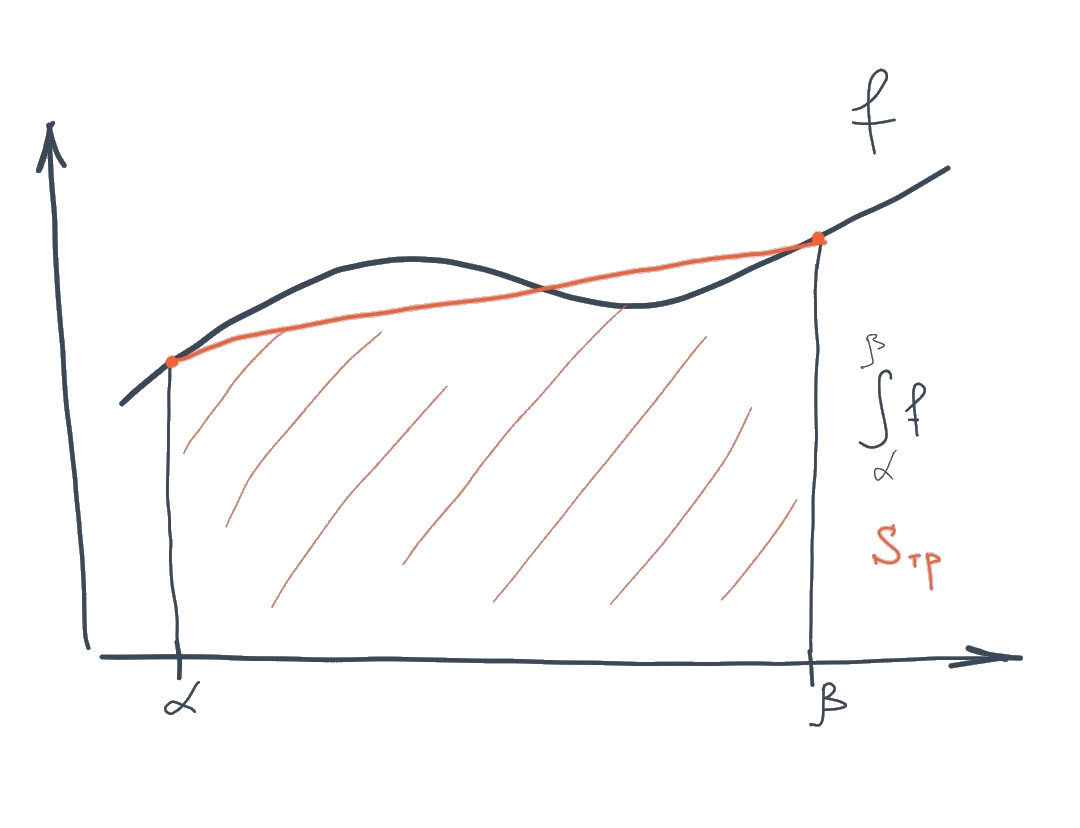
\includegraphics[scale=0.16]{riemann_trapezoid}
    \end{figure}
\end{remark}

\begin{theorem}[Оценка погрешности в формуле трапеции]
    Пусть $f \in C^2[a, b]$.

    Тогда : \[\left|\int\limits_a^b f(t) \mathrm{d}t - \sum_{k=1}^n \frac{f(x_{k-1}) + f(x_k)}{2}(x_k - x_{k-1})\right| \le \frac{|\tau|^2}{8} \int\limits_a^b |f''|\]
\end{theorem}
\begin{proof}
    $\Delta \coloneqq \int\limits_a^b - \sum \ldots = \sum\limits_{k=1}^n \int\limits_{x_{k-1}}^{x_k}f(t)\mathrm{d}t - \sum\limits_{k=1}^n \frac{f(x_{k-1}) + f(x_k)}{2}(x_k - x_{k-1})$

    \begin{align}
        |\Delta| \le  \sum\limits_{k=1}^n |\int\limits_{x_{k-1}}^{x_k} f(t)\mathrm{d}t - \frac{f(x_{k-1}) + f(x_k)}{2}(x_k - x_{k-1})| = \frac{1}{2} \sum\limits_{k=1}^n \left| \int_{x_{k-1}}^{x_k} f''(t)(t-x_{k-1})(x_k - t)\mathrm{d}t\right|
    .\end{align} Тогда вспомним, что $(t-x_{k-1})(x_k - t) \le \left( \frac{x_k - x_{k-1}}{2}\right)^2 \le \frac{|\tau|^2}{4} \implies (4) \le \frac{1}{2} \sum\limits_{k=1}^n\ \int\limits_{x_{k-1}}^{x_k}|f''(t)| \cdot \frac{|\tau|^2}{4} \mathrm{d}t = \frac{|\tau|^2}{8} \sum \int\limits_{x_{k-1}}^{x_k} |f''| = \frac{|\tau|^2}{8} \cdot \int\limits_a^b |f''|$
\end{proof}
\begin{remark}
    Пусть разбиение на $n$ равных отрезков  $x_k - x_{k-1} = \frac{b-a}{n} = |\tau|$:
    \[
        \sum_{k=1}^n \frac{f(x_{k-1}) + f(x_k)}{2}(x_k - x_{k-1}) = \frac{b-a}{n} \sum_{k=1}^n \frac{f(x_{k-1}) + f(x_k)}{2} = \frac{b-a}{n}(\frac{f(x_0)}{2} + \sum_{k=1}^{n-1}f(x_k) + \frac{f(x_n)}{2})
    .\] 
\end{remark}
\begin{remark}
    Возьмем разбиение на равные отрезки и $\xi_k = x_k$:
     \[
         S(f, \tau, \xi) = \sum_{k=1}^n f(\xi_k)(x_k - x_{k-1}) = \frac{b-a}{n} \sum_{k=1}^n f(x_k)
    .\] 
\end{remark}
%END TICKET 16